\section{Context-Free Parsing with CKY}

\textbf{Goal}: Find the syntax parsing tree of a context-free grammar. A constituent is a word or a group of words that function as a single unit within a hierarchical structure. Every node in the parsing tree is a constituent.
\vspace{-0.4cm}
\begin{center}
    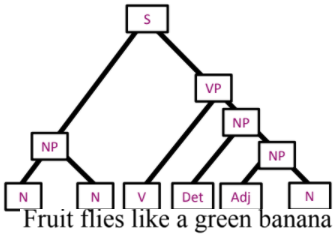
\includegraphics[width=.5\columnwidth]{img/syntex-tree.png}
\end{center}
\vspace{-0.4cm}
\subsection*{Context-Free Grammar}

Components: (1) Non-terminal symbol set, (2) a start non-terminal, (3) a set of terminal symbols and (4) a set of production rules.

A grammar is in Chomsky normal form if all production rules are of the form: $N_1\rightarrow N_2 N_3$, $N\rightarrow a$.

\subsection*{Probabilistic CFG}

Each production rule has a probability. The probability of a tree is computed by multiplying the probabilities of all the edges. PCFG is locally normalized, making the normalizer 1.

\subsection*{Weighted CFG}

Each production rule has a generic non-negative weight. The weights of trees are softmaxed to be a valid distribution. WCFG is globally normalized. In general, the output space is infinite, making computation of normalizer hard. However, we can efficiently compute the normalizer for a fixed sentence.

\subsection*{Parsing a string}

\vspace{-0.4cm}
$$p(t\mid s) = \frac{\exp(\text{score}(t))}{Z(s)}$$
\vspace{-0.3cm}

To avoid divergence of $Z(s)$ which could be caused by the infinite number of parsing trees, we can only look at trees in CNF because the CNF theorem says that for any grammar $G$, there is another grammar $G^\prime$ that accepts the same set of strings and is in CNF. The number of possible CNF parsing tree (each non-terminal symbol has two children and each terminal symbol has one leaf child) is $O(4^N)$, no longer infinite.

\subsection*{CKY Algorithm}

This algorithm finds all valid parsing trees under the given production rule set for CFG in CNF form in $O(N^3 |R|)$, where $N$ is the length of the string and $R$ is the rule set.

\vspace{-0.4cm}
\begin{center}
    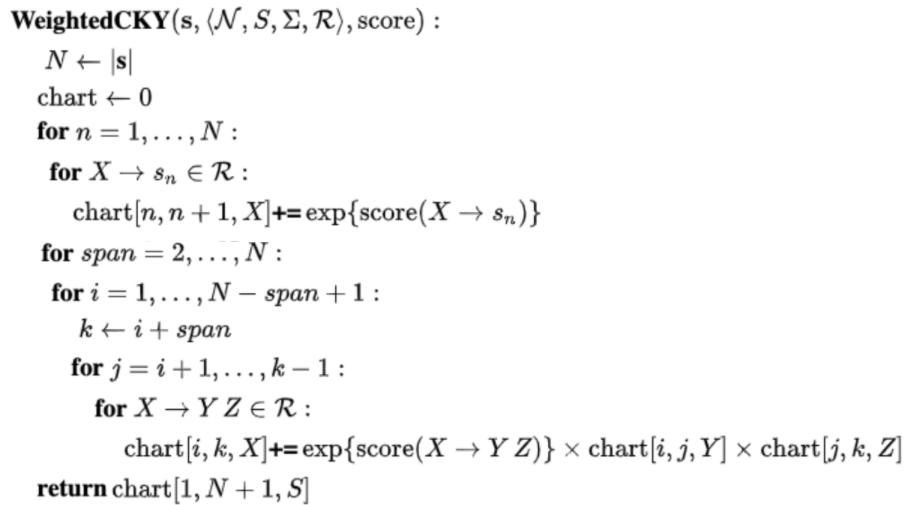
\includegraphics[width=\columnwidth]{img/CKY.png}
\end{center}
\vspace{-0.4cm}

Using the $(\max, \times)$ semiring decodes the best parsing.
